\documentclass[onecolumn, draftclsnofoot,10pt, compsoc]{IEEEtran}
\usepackage{graphicx}
\usepackage{url}
\usepackage{setspace}

\usepackage{geometry}
\geometry{textheight=9.5in, textwidth=7in}

\usepackage{graphicx}
\graphicspath{{images/}}

% 1. Fill in these details
\def \CapstoneTeamName{		Team Wombat}
\def \CapstoneTeamNumber{		15}
\def \GroupMemberOne{			Victor Li}
\def \GroupMemberTwo{			Ryan Crane}
\def \GroupMemberThree{			Nicholas Wong}
\def \CapstoneProjectName{		Axolotl}
\def \CapstoneSponsorCompany{	}
\def \CapstoneSponsorPerson{		Kevin McGrath}

% 2. Uncomment the appropriate line below so that the document type works
\def \DocType{		%Problem Statement
				Requirements Document
				%Technology Review
				%Design Document
				%Progress Report
				}
			
\newcommand{\NameSigPair}[1]{\par
\makebox[2.75in][r]{#1} \hfil 	\makebox[3.25in]{\makebox[2.25in]{\hrulefill} \hfill		\makebox[.75in]{\hrulefill}}
\par\vspace{-12pt} \textit{\tiny\noindent
\makebox[2.75in]{} \hfil		\makebox[3.25in]{\makebox[2.25in][r]{Signature} \hfill	\makebox[.75in][r]{Date}}}}
% 3. If the document is not to be signed, uncomment the RENEWcommand below
%\renewcommand{\NameSigPair}[1]{#1}

%%%%%%%%%%%%%%%%%%%%%%%%%%%%%%%%%%%%%%%
\begin{document}
\begin{titlepage}
    \pagenumbering{gobble}
    \begin{singlespace}
    	
\includegraphics[height=4cm]{coe_v_spot1}
        \hfill 
        % 4. If you have a logo, use this includegraphics command to put it on the coversheet.
        %\includegraphics[height=4cm]{CompanyLogo}   
        \par\vspace{.2in}
        \centering
        \scshape{
            \huge CS Capstone \DocType \par
            {\large\today}\par
            \vspace{.5in}
            \textbf{\Huge\CapstoneProjectName}\par
            \vfill
            {\large Prepared for}\par
            \Huge \CapstoneSponsorCompany\par
            \vspace{5pt}
            {\Large\NameSigPair{\CapstoneSponsorPerson}\par}
            {\large Prepared by }\par
            Group\CapstoneTeamNumber\par
            % 5. comment out the line below this one if you do not wish to name your team
            \CapstoneTeamName\par 
            \vspace{5pt}
            {\Large
                \NameSigPair{\GroupMemberOne}\par
                \NameSigPair{\GroupMemberTwo}\par
                \NameSigPair{\GroupMemberThree}\par
            }
            \vspace{20pt}
        }
        %\begin{abstract}
        % 6. Fill in your abstract    
   % Our project requires the development of software to run a car infotainment system alongside a black box data log. Our software will run on an Nvidia Jetson TX2 and should be able to execute basic media and navigation tasks while also logging data from a variety of sensors. The goal is to allow people to modernize older cars with an array of fresh sensors and an interactive software interface. To accomplish this goal, we will pull vehicle data from a car?s OBDII (On Board Diagnostics II) port as well as our own sensors wired into the TX2, and feed that data to software that aggregate that data into a log. 
      %  \end{abstract}     
    \end{singlespace}
\end{titlepage}
\newpage
\pagenumbering{arabic}
\tableofcontents
% 7. uncomment this (if applicable). Consider adding a page break.
%\listoffigures
%\listoftables
\clearpage

% 8. now you write!
\section{Introduction}
\subsection{Purpose}
The purpose of this software requirements specification (SRS) document is to outline and detail the capabilities of the NVIDIA Jetson TX2 infotainment and black box our group will develop, known henceforth as the Axolotl Infotainment System and Axolotl Software. Doing so will enable us to describe the requirements of the Axolotl Infotainment System and Axolotl Software such that we and our client will have a detailed understanding of the form factor and capabilities of the deliverable system we will develop. The intended audience for this SRS includes our client, the CS Capstone Instructors, and our group.\par

\subsection{Scope}
Our project entails the development of an infotainment system and black box that can be divided into two products: the Axolotl and the Axolotl Software. The Axolotl will connect vehicle sensors, controllers, receivers, and a touchscreen to a NVIDIA Jetson TX2 computer in a package that can be installed in a vehicle. The Axolotl Software runs on the Axolotl and provides users with media playback, navigation, and vehicle data logging capabilities.\par

\section{Definitions}
\begin{itemize}
	\item NVIDIA Jetson TX2: A versatile, efficient, and high-performance computer made by NVIDIA to be used in robots, drones, and smart cameras.

	\item OBD-II: On-Board Diagnostics II, a standardized connector installed in all automobiles sold in the United States since January 1st, 1996. Devices connected via a car's OBD-II port can read the vehicle's sensor data on the fly.
	
	\item CAN-bus: Controller Area Network Bus, a vehicle data system that allows sensors and microcontrollers to communicate with each other without a central computer.

	\item LIDAR: Light Detection and Ranging, a method of using laser pulses to determine the 3D properties of a faraway object.

	\item AHRS: Attitude, Heading, and Reference System, a system used in modern aircraft to determine and display roll, pitch, and yaw.

	\item Infotainment: A portmanteau of "��information" and "��entertainment"��. When we use the term "infotainment", we are referring to the center console touchscreen that gives drivers access to information and media in modern cars.

	\item RDS: Radio Data System, a method of transmitting the current track information of an FM radio broadcast.

	\item UPS: Uninterruptible Power Supply, an auxiliary power source that enables a device to function for a limited time if its main power source is unavailable.

\end{itemize}

\section{Overall Description}
\subsection{Product Perspective}
The Axolotl Infotainment System is comprised of the Axolotl Head Unit and the Axolotl Software.
The Axolotl Head Unit consists of all of the necessary sensors, receivers, and controller hardware connected physically and wirelessly with the NVIDIA Jetson TX2 system. The Axolotl is designed to be integrated into a car to either provide or replace an in-car infotainment system. Users will not interact directly with the sensors, receivers, or controllers.\par

The Axolotl Software will be installed on the Axolotl Head Unit's TX2 unit and directly interface with the user. The software will operate on Linux, as it is the base operating system installed on the TX2. The Axolotl Software will interact with the hardware and provide users with the ability to control media playback, conduct mapping and routing with navigation, and also exert limited control over system settings.\par

\subsection{Product Functions}
The main functions of the Axolotl are:
\begin{itemize}
	\item	The Axolotl will allow users to play media from multiple sources including: USB, Bluetooth, Auxiliary, and FM.
	\item	It will also offer navigation with destination entry, mapping, and offline capabilities. 
	\item	The black box portion of the Axolotl logs output from a dashcam and all sensors tied into a car's OBD-II port. Users are able to download the black box data to a storage device or clear all black box data. 
	\item	The Axolotl display will also switch to the backup camera whenever user is reversing the car.
	
\end{itemize}
\subsection{User Interfaces}
The Axolotl Software will be interacted via a touchscreen using an iOS-inspired graphical user interface divided into the content window and the dock. The dock offers touch zones that will change the content window to either the media, navigation, or system menu. Each content window will have a submenu that displays contextual options and a content box encapsulating the main interactive content that changes based on the option selected in the submenu.\par
\subsection{Hardware Interfaces}
The hardware components of the system will include: the use of OBII which will receive information from multiple onboard car sensors, all related audio connection capabilities (which includes radio, bluetooth, auxiliary, and USB), the storing of data for navigation, and logging of all sensor data from the car in hard drives. The NVIDIA TX2 has native support for all hardware that is being used. \par
\subsection{User Characteristics}
The Axolotl will be used by ourselves, our client, and the general public, specifically car owners with any level of technological experience.\par
\subsection{Constraints}
\begin{itemize}
	\item Hardware limitations including input, memory space, and form factor
	\item Entertainment to be limited as to not cause distraction
\end{itemize}
\subsection{Assumptions}
\begin{itemize}
	\item This SRS assumes the availability of an accessible WiFi network with internet connectivity.
	\item This SRS assumes the availability of GPS signal.
	\item This SRS assumes the TX2 runs Linux.
\end{itemize}
\section{Specific Requirements}
\subsection{External Interfaces}
Axlotl Software
\begin{itemize}
	\item The Axolotl Software is a Linux program that is installed on the NVIDIA Jetson TX2.
	\item Users interact with the Axolotl via a graphic user interface displayed on a touchscreen.
	\begin{itemize}
		\item Users are able to operate Media, Navigation, and system settings, and may switch between them at any time.
	\end{itemize}
	\item Users may set either FM, Aux, USB, or Bluetooth as the audio source. 
	\begin{itemize}
		\item Users may change the current FM radio frequency.
		\item Users may control pause/play/previous track/next track functionality with USB and Bluetooth media sources via the touchscreen.
		\item All media options will offer a volume slider for users to adjust global audio output volume.
	\end{itemize}
	\item Users may utilize map, destination entry, and view route Navigation functions.
	\begin{itemize}
		\item Users may input an address to set the destination of the routing system.
	\end{itemize}
	\item Users may turn off the system's WiFi connectivity by a toggle switch.
	\item Users may download or wipe black box data by selecting the Black Box option.
\end{itemize}
\subsection{Functions}
\subsection{Axolotl Software}
\begin{itemize}
	\item Users will be able to see radio broadcast information within the FM media option will display RDS data.
	\item The Aux media option will indicate that media playback is controlled by the connected aux device.
	\item The USB media option will allow for full exploration of the connected USB drive's file structure.
	\begin{itemize}
		\item Playback of mp3s is supported.
	\end{itemize}
	\item The system shall record vehicle data from an OBD-II port, connected dashcam, and AHRS onto a SATA drive.
	\item Navigation will be capable of routing and mapping even if a mobile data signal is not available. Navigation will also parse address strings entered for destination input into a valid destination address for routing. The system will alert the user if the address entered is invalid.
	\item Navigation will utilize a single GPS receiver unit to determine location.
	\item The Navigation system will be limited to addresses within the United States.
	\item Users must enter a password in order to interact with the Black Box option within the System menu.
	\item The display will automatically switch to the backup camera feed when the vehicle is reversing. 
	\item The Axolotl implementation will offer a minimum of three of any of the following optional functions:
	\begin{itemize}
		\item Display of current driving statistics to improve driver's habits.
		\item Use of multiple GPS receivers throughout the vehicle to improve accuracy of GPS location.
		\item Display of live AHRS data in a System submenu.
		\item Control over supplemental turn signals and backup lights managed by a wireless controller in order to better signal other drivers.
		\item Topographical maps option of surroundings in navigation.
		\item Users can utilize a file browser to wirelessly download media from a home computer to a USB drive connected to the Axolotl.
		\item Physical knobs for volume and radio.
		\item Bluetooth calling support.
		\item Dashcam lane departure warning.
		\item Use of LIDAR to assist parking.
		\end{itemize}
\end{itemize}
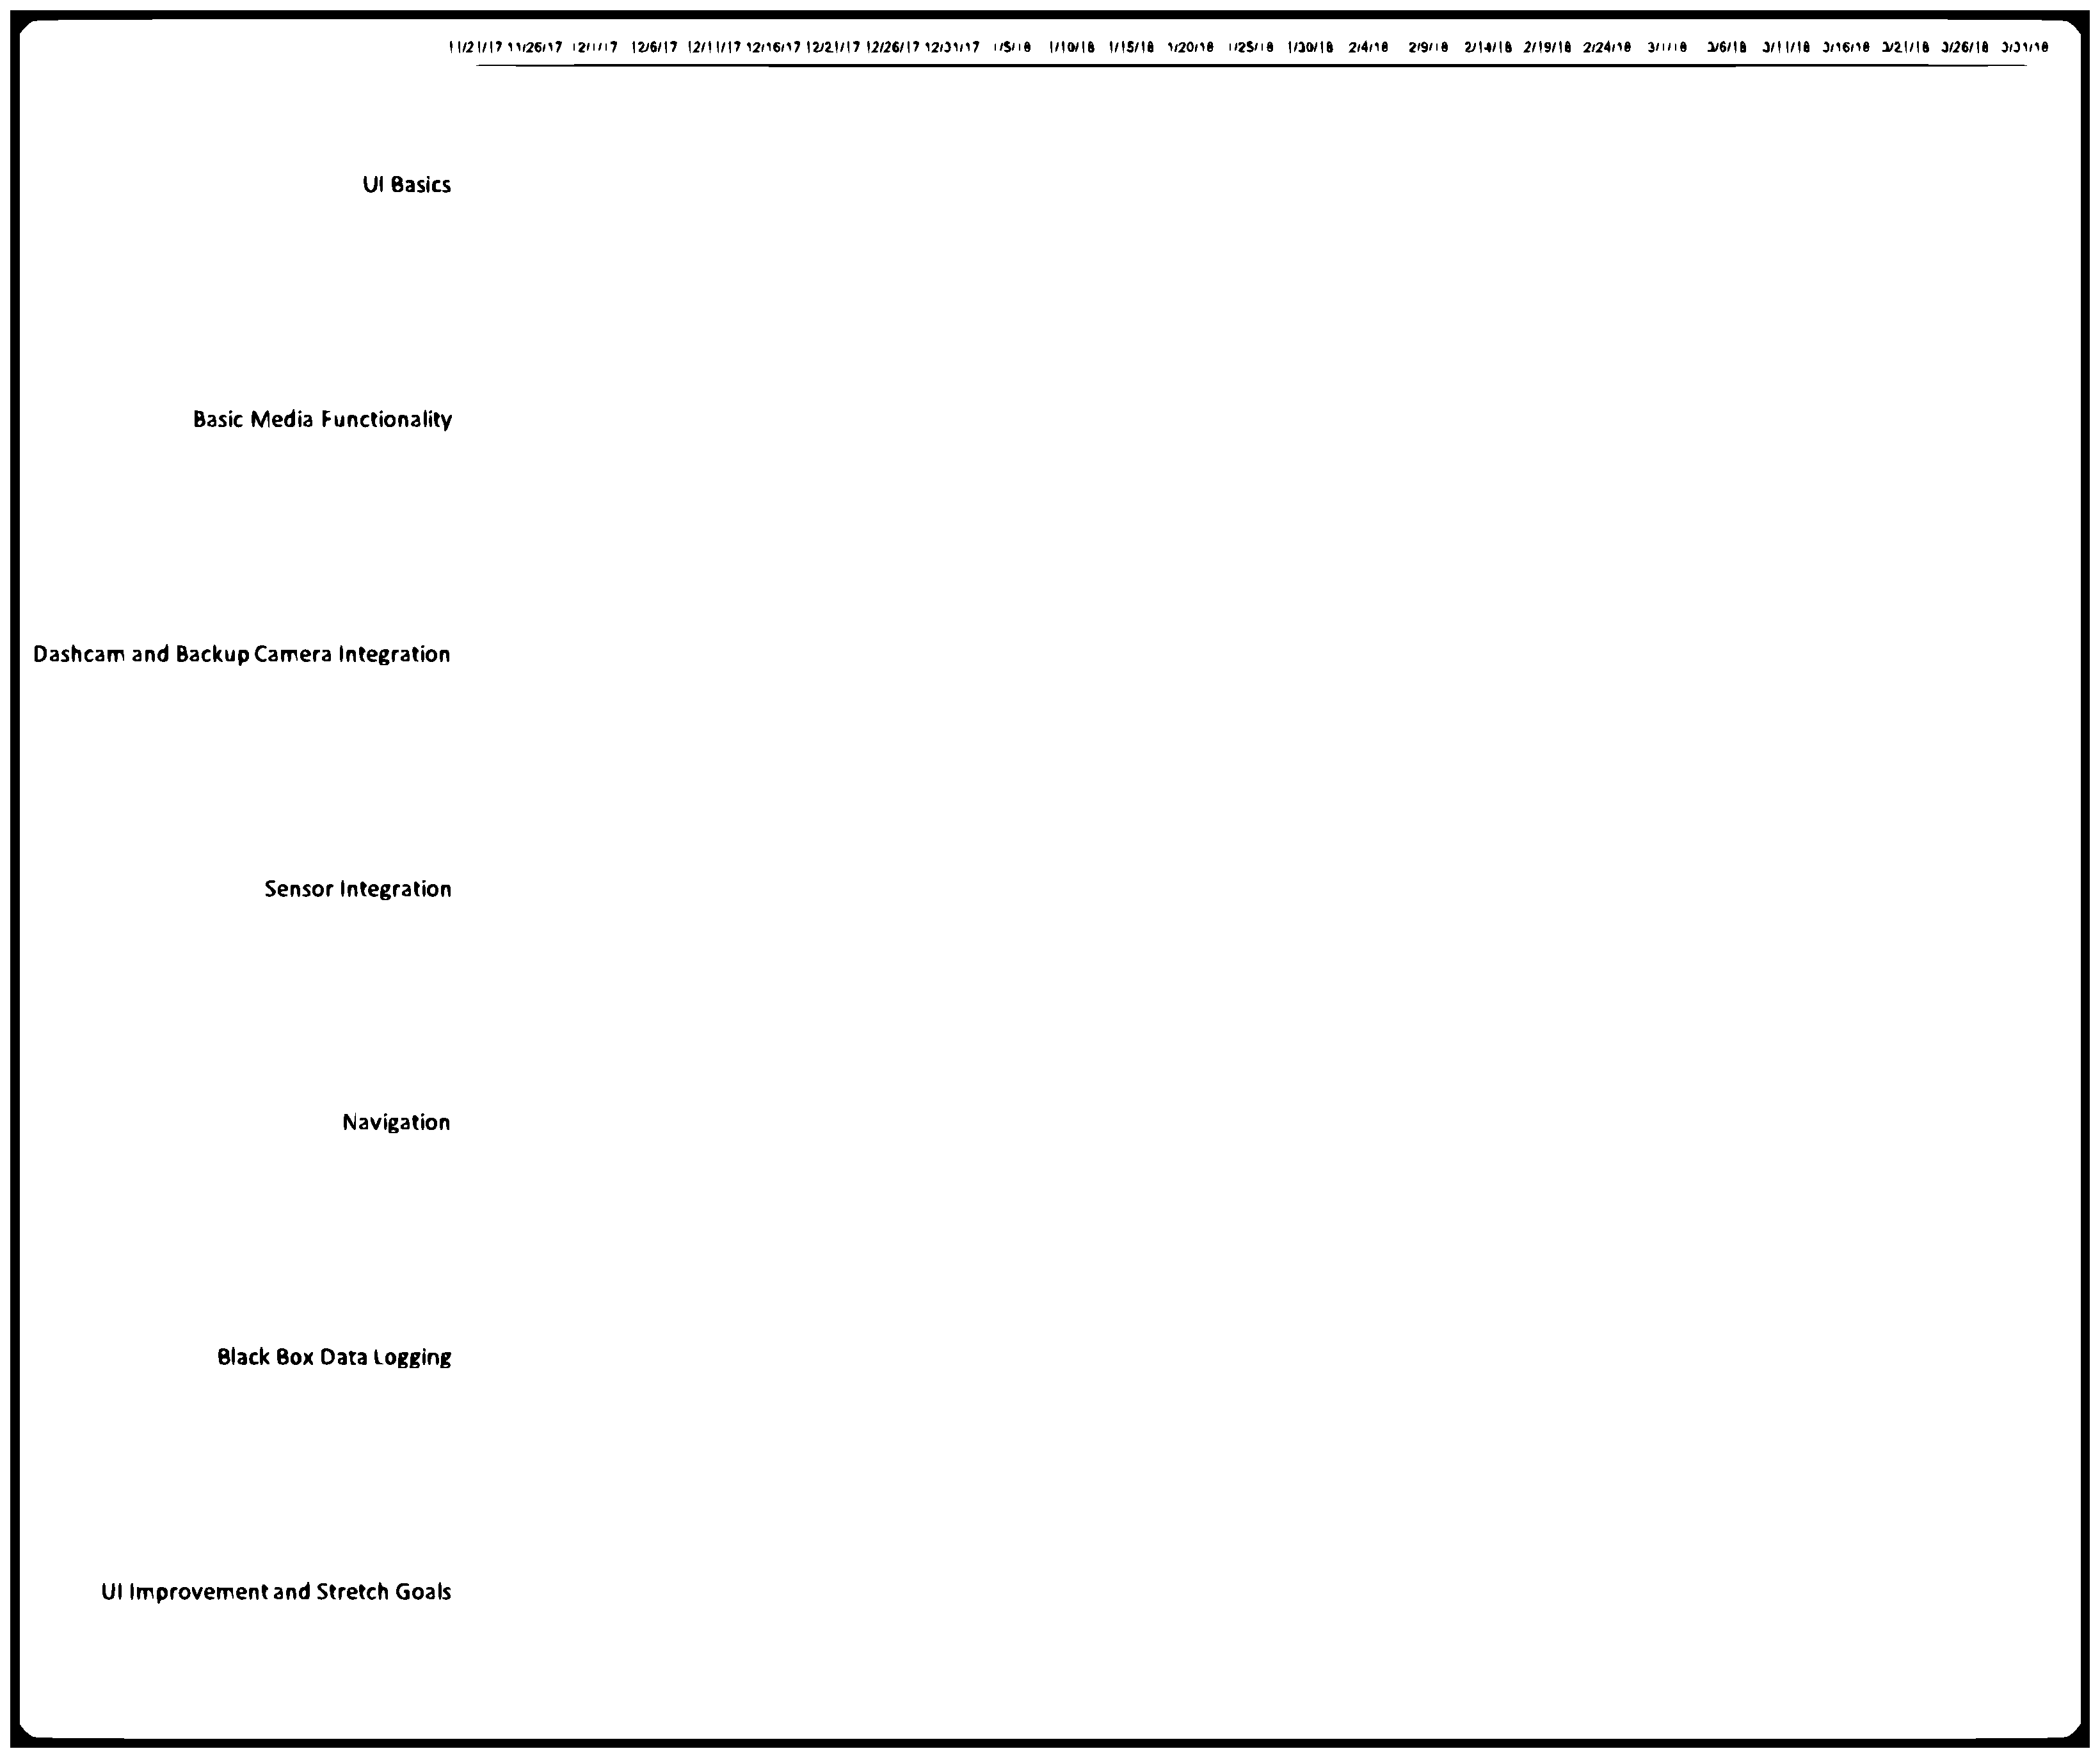
\includegraphics[width=\textwidth ]{gantt.eps}
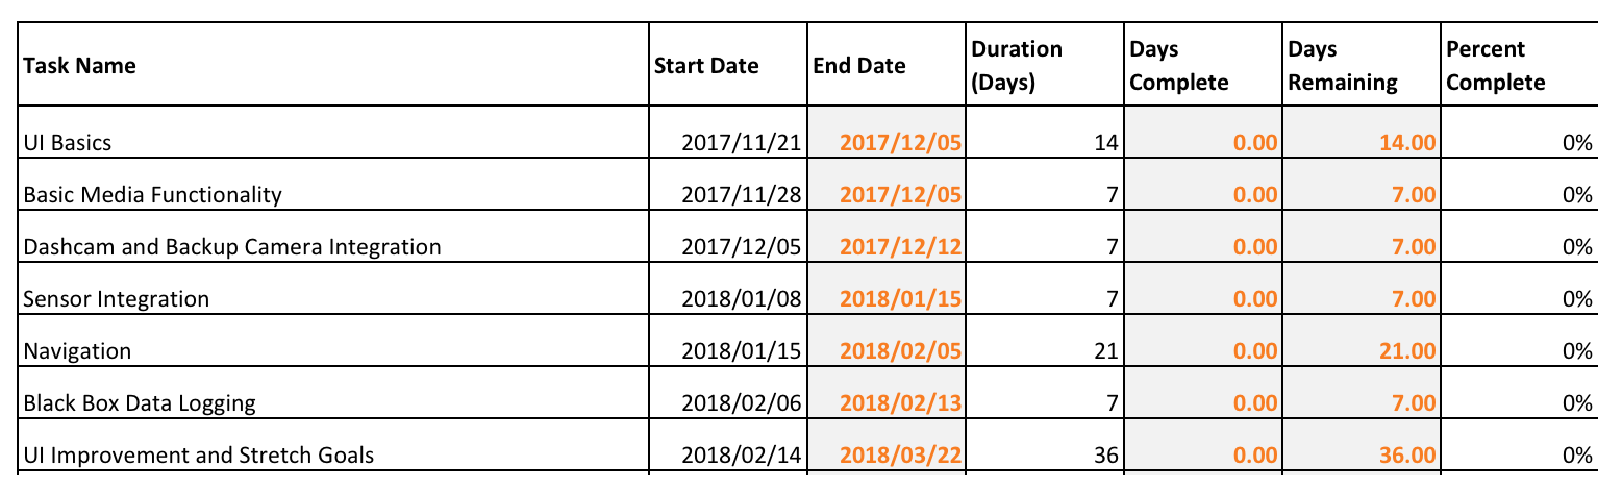
\includegraphics[width=\textwidth]{tablegantt.eps}
\end{document}
